\documentclass[aspectratio=169,11pt]{beamer}

% ============================================================
% Theme & Colors
% ============================================================
\usetheme{metropolis}
\usepackage{appendixnumberbeamer}

% ANU-inspired color palette
\definecolor{anuGold}{RGB}{190,163,96}
\definecolor{postechBlue}{RGB}{0,51,102}
\definecolor{accentBlue}{RGB}{59,130,246}
\definecolor{lightGray}{RGB}{245,245,250}
\definecolor{darkText}{RGB}{30,30,50}
\definecolor{mutedText}{RGB}{100,100,120}

\setbeamercolor{frametitle}{bg=postechBlue, fg=white}
\setbeamercolor{title}{fg=postechBlue}
\setbeamercolor{progress bar}{fg=anuGold, bg=postechBlue!20}
\setbeamercolor{alerted text}{fg=accentBlue}
\setbeamercolor{block title}{bg=postechBlue, fg=white}
\setbeamercolor{block body}{bg=lightGray}
\setbeamercolor{section in toc}{fg=postechBlue}

\setbeamerfont{title}{series=\bfseries, size=\Large}
\setbeamerfont{frametitle}{series=\bfseries}

% ============================================================
% Packages
% ============================================================
\usepackage{booktabs}
\usepackage{graphicx}
\usepackage{tikz}
\usetikzlibrary{arrows.meta, positioning, shapes, calc, decorations.pathreplacing}
\usepackage{xcolor}
\usepackage{hyperref}
\usepackage{fontawesome5}
\usepackage{multicol}

% ============================================================
% Custom Commands
% ============================================================
\newcommand{\paperref}[3]{\textbf{#1} \hfill {\small\color{mutedText}#2 #3}}
\newcommand{\papercite}[1]{{\scriptsize\color{mutedText}#1}}
\newcommand{\highlight}[1]{\textcolor{accentBlue}{\textbf{#1}}}
\newcommand{\venue}[1]{{\small\textcolor{postechBlue}{\textbf{#1}}}}
\newcommand{\badge}[1]{\colorbox{anuGold}{\scriptsize\color{white}\textbf{#1}}}
\newcommand{\anucollab}{\faHandshake~\textcolor{anuGold}{\scriptsize ANU Collab}}

% ============================================================
% Title Information
% ============================================================
\title{The Structure Beneath}
\subtitle{How Geometry and Graphs Shape What Models Can Learn}
\author{Dongwoo Kim}
\institute{
  Department of Computer Science \& Engineering \\
  Graduate School of AI \\
  POSTECH (Pohang University of Science and Technology)
}
\date{Sabbatical Talk at ANU \\ February 2026}

% ============================================================
\begin{document}
% ============================================================

% ------ Title ------
\maketitle

% ============================================================
% OPENING
% ============================================================
\section{Introduction}

% ------ About Me ------
\begin{frame}{About Me}
\begin{columns}[T]
\begin{column}{0.55\textwidth}
  \textbf{Dongwoo Kim} \\[3pt]
  Associate Professor, POSTECH \\
  CSE \& Graduate School of AI \\[6pt]
  {\small
  \begin{itemize}\setlength\itemsep{1pt}
    \item PhD, KAIST (2015) --- Topic Models, NLP
    \item Postdoc \& Lecturer, ANU (2015--2019)
    \item Assistant $\to$ Associate Prof, POSTECH (2019--)
    \item Honorary Lecturer, ANU (2019--2024)
    \item Visiting Researcher, ANU (2026)
  \end{itemize}
  }
\end{column}
\begin{column}{0.4\textwidth}
  \centering
  % Placeholder for photo
  
\begin{tikzpicture}
    \draw[rounded corners=8pt, fill=lightGray, draw=postechBlue, thick]
      (0,0) rectangle (3.5,4);
    \node[text=mutedText] at (1.75,2) {\Large Photo};
  \end{tikzpicture}
\end{column}
\end{columns}
\end{frame}

% ------ POSTECH ML Lab ------
\begin{frame}{POSTECH Machine Learning Lab}
\small
\begin{columns}[T]
\begin{column}{0.48\textwidth}
  \textbf{PhD \& Combined Students}
  \begin{itemize}\setlength\itemsep{0pt}
    \item Moonjeong Park {\scriptsize -- GNNs, Dynamical Systems}
    \item Seungbeom Lee {\scriptsize -- Geometric DL, ML for Bio}
    \item Seunghyuk Cho {\scriptsize -- Generative, Riemannian}
    \item Jaeseung Heo {\scriptsize -- GNNs, Data-Centric AI}
    \item Saemi Moon {\scriptsize -- Trustworthy AI}
    \item Youngbin Choi {\scriptsize -- LLM Personalization}
    \item Minjong Lee {\scriptsize -- Generative Models}
  \end{itemize}
\end{column}
\begin{column}{0.48\textwidth}
  \textbf{PhD Students (cont.)}
  \begin{itemize}\setlength\itemsep{0pt}
    \item Kyeongheung Yun {\scriptsize -- GNNs}
    \item Seokwon Yoon {\scriptsize -- Machine Learning}
    \item Chongtae Ahn {\scriptsize -- ML (Industrial, POSCO)}
  \end{itemize}
  \vspace{6pt}
  \textbf{MS Students}
  \begin{itemize}\setlength\itemsep{0pt}
    \item Yesong Ko {\scriptsize -- Machine Learning}
    \item Sunghyun Choi {\scriptsize -- ML, Generative Models}
  \end{itemize}
\end{column}
\end{columns}
\end{frame}

% ------ ANU Connections ------
\begin{frame}{A Long History with ANU}
\vspace{-4pt}
\begin{center}
  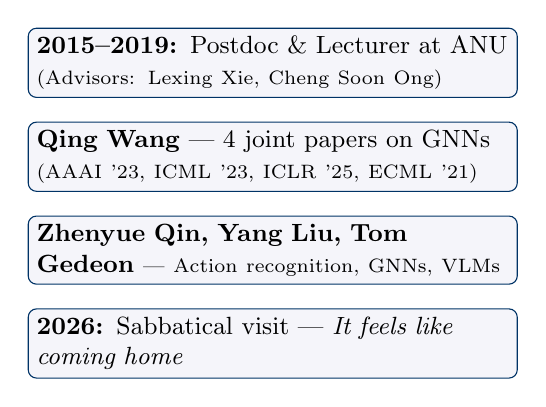
\begin{tikzpicture}[
    node distance=0.3cm,
    every node/.style={font=\small},
    event/.style={draw=postechBlue, rounded corners=3pt, fill=lightGray,
                  text width=6cm, align=left, inner sep=3pt, font=\small}
  ]
    \node[event] (e1) {
      \textbf{2015--2019:} Postdoc \& Lecturer at ANU
      {\scriptsize (Advisors: Lexing Xie, Cheng Soon Ong)}
    };
    \node[event, below=of e1] (e2) {
      \textbf{Qing Wang} --- 4 joint papers on GNNs
      {\scriptsize (AAAI '23, ICML '23, ICLR '25, ECML '21)}
    };
    \node[event, below=of e2] (e3) {
      \textbf{Zhenyue Qin, Yang Liu, Tom Gedeon}
      {\scriptsize --- Action recognition, GNNs, VLMs}
    };
    \node[event, below=of e3] (e4) {
      \textbf{2026:} Sabbatical visit --- \textit{It feels like coming home}
    };
  \end{tikzpicture}
\end{center}
\end{frame}

% ------ Framing: The Journey ------
\begin{frame}{The Journey}
\begin{center}
  {\large\textcolor{postechBlue}{\textit{``How should we represent, learn from, and control structured knowledge?''}}}
\end{center}
\vspace{4pt}
\begin{center}
  {\small Structure is both the \alert{solution} and the \alert{problem}.\\
  Graphs encode relations, geometry captures hierarchy, symmetry constrains models ---\\
  but structure also introduces over-smoothing, noise propagation, and hidden bias.}
\end{center}
\vspace{6pt}

\begin{center}
  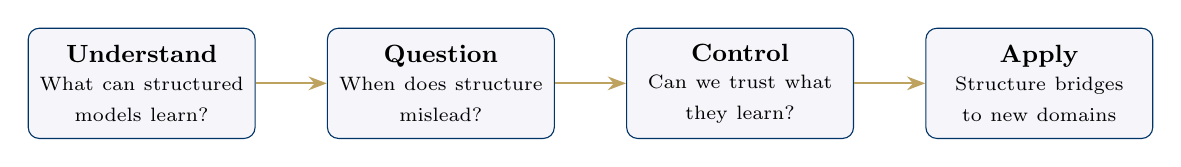
\begin{tikzpicture}[
    act/.style={draw=postechBlue, rounded corners=4pt, fill=lightGray,
                minimum width=2.8cm, minimum height=1.4cm, align=center,
                font=\small, text width=2.6cm, inner sep=4pt}
  ]
    \node[act] (a1) at (0,0) {
      \textbf{Understand}\\[2pt]
      {\scriptsize What can structured\\models learn?}
    };
    \node[act] (a2) at (3.8,0) {
      \textbf{Question}\\[2pt]
      {\scriptsize When does structure\\mislead?}
    };
    \node[act] (a3) at (7.6,0) {
      \textbf{Control}\\[2pt]
      {\scriptsize Can we trust what\\they learn?}
    };
    \node[act] (a4) at (11.4,0) {
      \textbf{Apply}\\[2pt]
      {\scriptsize Structure bridges\\to new domains}
    };

    \draw[-{Stealth}, thick, anuGold] (a1) -- (a2);
    \draw[-{Stealth}, thick, anuGold] (a2) -- (a3);
    \draw[-{Stealth}, thick, anuGold] (a3) -- (a4);
  \end{tikzpicture}
\end{center}

\vspace{4pt}
\begin{center}
  {\small $\sim$20 papers at top venues (NeurIPS, ICML, ICLR, ICCV, EMNLP, AAAI, \ldots)}
\end{center}
\end{frame}

% ============================================================
% ACT 1: Understand
% ============================================================
\section{Act 1: What Can Structure-Aware Models Learn?}

% ------ Expressivity: Vertex Colouring ------
\begin{frame}{Breaking the Expressivity Barrier}
  \papercite{Shouheng Li, Dongwoo Kim, Qing Wang \hfill \venue{ICML 2023} \anucollab}
  \vspace{8pt}

  \textbf{The challenge:} Standard message-passing GNNs are bounded by the \alert{1-WL test}
  \vspace{6pt}

  \textbf{Key idea:} Use \alert{local vertex colouring} to break symmetry
  \begin{itemize}
    \item Assign initial colours based on local structure
    \item GNNs with vertex colouring distinguish graphs beyond 1-WL
    \item Higher expressivity \textit{without} expensive higher-order message passing
  \end{itemize}
  \vspace{8pt}

  \textbf{Result:} More expressive GNNs that remain practically efficient

  % Placeholder for figure
  \begin{center}
    {\small\color{mutedText}[Figure: Vertex colouring illustration]}
  \end{center}
\end{frame}

% ------ Heterophily: Restructuring ------
\begin{frame}{When Structure Hinders: Heterophilic Graphs}
  \papercite{Shouheng Li, Dongwoo Kim, Qing Wang \hfill \venue{AAAI 2023} \anucollab}
  \vspace{8pt}

  \textbf{The problem:} GNNs assume neighbours are similar --- but what if they're \alert{not}?
  \vspace{6pt}

  Heterophilic graphs violate the homophily assumption underlying most GNNs
  \vspace{4pt}

  \textbf{Key idea:} Don't fight the graph --- \textit{restructure} it
  \begin{itemize}
    \item Learnable spectral clustering rewires edges
    \item Increases effective homophily ratio
    \item GNN then operates on a friendlier graph topology
  \end{itemize}
  \vspace{8pt}

  \textbf{Result:} Significant gains on heterophilic benchmarks

  % Placeholder for figure
  \begin{center}
    {\small\color{mutedText}[Figure: Graph restructuring pipeline]}
  \end{center}
\end{frame}

% ------ Bridging Theory + Qing Memorial ------
\begin{frame}{Bridging Expressivity and Generalization}
  \papercite{Shouheng Li, Floris Geerts, Dongwoo Kim, Qing Wang \hfill \venue{ICLR 2025} \anucollab}
  \vspace{8pt}

  \textbf{Core question:} Is there a fundamental trade-off between expressivity and generalization?
  \vspace{6pt}

  \textbf{Key contributions:}
  \begin{itemize}
    \item Unified framework connecting WL hierarchy (expressivity) with Rademacher complexity (generalization)
    \item Higher expressivity need \textit{not} hurt generalization
    \item Practical guidelines for principled GNN architecture design
  \end{itemize}
  \vspace{6pt}

  \begin{block}{}
    \centering
    \textit{In loving memory of our collaborator and friend, Qing Wang.}\\
    {\scriptsize Four papers together --- this line of work is her legacy too.}
  \end{block}
\end{frame}

% ------ Transition to Act 2 ------
\begin{frame}[plain]
  \vspace{2cm}
  \begin{center}
    {\Large\textcolor{postechBlue}{Theory says GNNs are powerful ---}}\\[8pt]
    {\Large\textcolor{postechBlue}{but practitioners see degradation in deep networks.}}\\[16pt]
    {\large\textcolor{mutedText}{What's going wrong?}}
  \end{center}
\end{frame}

% ============================================================
% ACT 2: When Structure Misleads
% ============================================================
\section{Act 2: When Structure Misleads}

% ------ Reverse Process GNN ------
\begin{frame}{Turning Smoothing into a Feature}
  \papercite{MoonJeong Park, Jaeseung Heo, Dongwoo Kim \hfill \venue{ICML 2024}}
  \vspace{8pt}

  \textbf{Insight:} Message passing is a \alert{diffusion process} --- can we \textit{reverse} it?
  \vspace{6pt}

  \begin{itemize}
    \item Standard GNNs: forward diffusion $\to$ smoothing $\to$ information loss
    \item Our approach: learn a \textit{reverse} diffusion process
    \item Recovers discriminative node features even on heterophilic graphs
    \item Principled framework connecting diffusion models with GNNs
  \end{itemize}
  \vspace{8pt}

  \textbf{Result:} State-of-the-art on heterophilic benchmarks while maintaining homophilic performance

  % Placeholder for figure
  \begin{center}
    {\small\color{mutedText}[Figure: Forward vs.\ reverse diffusion on graphs]}
  \end{center}
\end{frame}

% ------ Posterior Label Smoothing ------
\begin{frame}{Working \textit{With} Structure, Not Against It}
  \papercite{Jaeseung Heo, Moonjeong Park, Dongwoo Kim \hfill \venue{AAAI 2026} \badge{Oral}}
  \vspace{8pt}

  \textbf{Instead of reversing smoothing --- what if we smooth \textit{smarter}?}
  \vspace{6pt}

  \textbf{Key idea:} \alert{Posterior} label smoothing for node classification
  \begin{itemize}
    \item Smooth labels using graph-structure-aware posterior distribution
    \item Adapts smoothing strength based on local neighbourhood
    \item Theoretically principled: connects to Bayesian label propagation
  \end{itemize}
  \vspace{8pt}

  \textbf{Result:} Consistent improvements across homophilic \textit{and} heterophilic graphs

  \vspace{4pt}
  {\small\textit{From fighting structure to collaborating with it --- an evolving perspective.}}
\end{frame}

% ------ Oversmoothing Fallacy ------
\begin{frame}{The Oversmoothing Fallacy}
  \papercite{MoonJeong Park, Sunghyun Choi, Jaeseung Heo, Eunhyeok Park, Dongwoo Kim \hfill {\small\color{mutedText}arXiv}}
  \vspace{8pt}

  \textbf{Provocative claim:} Over-smoothing may be a \alert{misguided narrative}
  \vspace{6pt}

  Careful empirical study reveals:
  \begin{itemize}
    \item Performance degradation in deep GNNs is \textit{not} always due to over-smoothing
    \item Optimization issues (vanishing gradients, training instability) are often the real culprit
    \item Standard metrics for over-smoothing can be misleading
  \end{itemize}
  \vspace{8pt}

  \textbf{The arc:} Reverse it (ICML'24) $\to$ Work with it (AAAI'26) $\to$ Maybe it's not even the problem

  \vspace{4pt}
  {\small\textit{Sometimes the most important contribution is questioning the question itself.}}
\end{frame}

% ------ Data-Centric: Augmentation & Influence ------
\begin{frame}{The Model Is Only as Good as Its Data}
  \textbf{If imperfect structure corrupts learning, what about imperfect \textit{data}?}
  \vspace{8pt}

  \papercite{Jaeseung Heo*, Seungbeom Lee*, Sungsoo Ahn, Dongwoo Kim \hfill \venue{IJCAI 2024}}
  \vspace{2pt}
  \textbf{EPIC: Graph Augmentation via Edit Path Interpolation}
  \begin{itemize}
    \item Define augmentation via \alert{edit path interpolation} between graphs
    \item Generates structurally diverse yet semantically consistent graphs
  \end{itemize}

  \vspace{8pt}

  \papercite{Jaeseung Heo, Kyeongheung Yun, Seokwon Yoon, MoonJeong Park, Jungseul Ok, Dongwoo Kim \hfill \venue{NeurIPS 2025}}
  \vspace{2pt}
  \textbf{Influence Functions for Edge Edits in GNNs}
  \begin{itemize}
    \item Extend \alert{influence functions} to edge-level edits in non-convex GNNs
    \item Which edges matter most? Efficiently approximate the effect of adding/removing edges
  \end{itemize}
\end{frame}

% ------ Label Noise ------
\begin{frame}{When Labels Lie: Noise Propagation in Graphs}
  \papercite{Suyeon Kim, SeongKu Kang, Dongwoo Kim, Jungseul Ok, Hwanjo Yu \hfill \venue{KDD 2025}}
  \vspace{8pt}

  \textbf{Gap:} Instance-dependent label noise is well-studied for images, not for graphs
  \vspace{6pt}

  \begin{itemize}
    \item Noise patterns in graphs are fundamentally different from i.i.d.\ data
    \item Graph structure both \textit{propagates} and \textit{helps correct} label noise
    \item Comprehensive benchmark for evaluating robustness to label noise in GNNs
  \end{itemize}
  \vspace{8pt}

  \textbf{Shared insight across all three works:}\\
  {\small Augment what's missing (EPIC), measure what matters (influence), and understand how errors spread (label noise). \textit{Data quality is a structural problem.}}
\end{frame}

% ------ Transition to Act 3 ------
\begin{frame}[plain]
  \vspace{2cm}
  \begin{center}
    {\Large\textcolor{postechBlue}{If imperfect data corrupts learning,}}\\[8pt]
    {\Large\textcolor{postechBlue}{what happens when we \textit{need} to remove data?}}\\[16pt]
    {\large\textcolor{mutedText}{And how do we verify our models are actually robust?}}
  \end{center}
\end{frame}

% ============================================================
% ACT 3: Can We Trust What Structured Models Learn?
% ============================================================
\section{Act 3: Can We Trust What Structured Models Learn?}

% ------ Unlearning: Data Points to Features ------
\begin{frame}{Making Models Forget: From Data Points to Features}
  \textbf{The same team, an increasingly ambitious question}
  \vspace{8pt}

  \papercite{Youngsik Yoon*, Jinhwan Nam*, Jaeho Lee, Dongwoo Kim, Jungseul Ok \hfill \venue{IEEE S\&P 2024}}
  \vspace{2pt}
  \textbf{Few-shot Unlearning}
  \begin{itemize}
    \item Remove data influence with access to only a \alert{few samples}
    \item Provable guarantees on forgetting quality
    \item Published at S\&P --- bridging ML and security
  \end{itemize}

  \vspace{8pt}

  \papercite{Saemi Moon, Seunghyuk Cho, Dongwoo Kim \hfill \venue{AAAI 2024}}
  \vspace{2pt}
  \textbf{Feature Unlearning for Generative Models}
  \begin{itemize}
    \item Go beyond data points: unlearn \alert{features} from GANs and VAEs
    \item E.g., remove ability to generate glasses on faces
    \item Feature-level unlearning is more natural for generative models
  \end{itemize}
\end{frame}

% ------ HUB: Unlearning at Scale ------
\begin{frame}{From Features to Concepts: Unlearning at Scale}
  \papercite{Saemi Moon*, Minjong Lee*, Sangdon Park, Dongwoo Kim \hfill \venue{ICCV 2025}}
  \vspace{8pt}

  \textbf{How do we properly evaluate unlearning for text-to-image models?}
  \vspace{6pt}

  \textbf{HUB: Holistic Unlearning Benchmark}
  \begin{itemize}
    \item Evaluates along multiple axes:
    \begin{itemize}
      \item[-] Forgetting quality --- is the concept truly removed?
      \item[-] Generation quality --- does the model still work well?
      \item[-] Robustness --- can unlearning be circumvented?
    \end{itemize}
    \item Reveals surprising failure modes in existing methods
  \end{itemize}
  \vspace{8pt}

  \textbf{The unlearning arc:} Data points (S\&P'24) $\to$ Features (AAAI'24) $\to$ Concepts \& evaluation (ICCV'25)

  \vspace{4pt}
  {\small\textit{Each step raised the stakes --- and the bar for verification.}}
\end{frame}

% ------ Robustness ------
\begin{frame}{Rigorous Evaluation as a Contribution}
  \papercite{Minjong Lee, Dongwoo Kim \hfill \venue{ICCV 2023} \badge{Oral}}
  \vspace{8pt}

  \textbf{Context:} Diffusion-based purification claimed strong adversarial robustness
  \vspace{6pt}

  \textbf{Our finding:} Previous evaluations were \alert{fundamentally flawed}
  \begin{itemize}
    \item Gradient-based attacks fail due to stochastic purification process
    \item We design proper evaluation methodology with stronger attack protocols
    \item Robustness claims were significantly overstated
  \end{itemize}
  \vspace{8pt}

  \textbf{Lesson:} Rigorous evaluation is as important as strong defences

  \vspace{4pt}
  {\small Selected as \badge{Oral} at ICCV 2023 --- the community recognized that\\
  \textit{proving something doesn't work} can be the most valuable contribution.}
\end{frame}

% ------ Fairness ------
\begin{frame}{Bias Hides in Structure Too}
\begin{columns}[T]
\begin{column}{0.48\textwidth}
  \textbf{Fair Music Recommendation} \\
  \papercite{Jinhyeok Park*, Dain Kim*, Dongwoo Kim} \\
  \venue{CIKM 2022} \badge{Best Paper} \\[6pt]
  \begin{itemize}
    \item Item-based VAE for fair recommendation
    \item Mitigates popularity bias while maintaining quality
    \item Won Best Paper at EvalRS Data Challenge
  \end{itemize}
\end{column}
\begin{column}{0.48\textwidth}
  \textbf{ChronoBias for LLMs} \\
  \papercite{Kyungmin Kim, Youngbin Choi, Hyounghun Kim, Dongwoo Kim, Sangdon Park} \\
  \venue{EMNLP Findings 2025} \\[6pt]
  \begin{itemize}
    \item Benchmark for time-conditional group bias
    \item LLMs reflect biases from specific time periods
    \item First systematic study of temporal bias
  \end{itemize}
\end{column}
\end{columns}
\vspace{6pt}
{\small\textit{Bias is structural: it lives in recommendation graphs and temporal data distributions alike.}}
\end{frame}

% ------ Transition to Act 4 ------
\begin{frame}[plain]
  \vspace{2cm}
  \begin{center}
    {\Large\textcolor{postechBlue}{The principles we've developed ---}}\\[6pt]
    {\large\textcolor{postechBlue}{respect geometry, question assumptions, verify rigorously ---}}\\[12pt]
    {\Large\textcolor{mutedText}{apply far beyond graphs.}}
  \end{center}
\end{frame}

% ============================================================
% ACT 4: Structure as Bridge to New Domains
% ============================================================
\section{Act 4: Structure as Bridge to New Domains}

% ------ Hyperbolic: Consolidated ------
\begin{frame}{Matching Geometry to Data: Hyperbolic Representations}
  \textbf{When Euclidean space isn't enough:} Hierarchical data needs \alert{hyperbolic} geometry
  \vspace{8pt}

  \papercite{Seunghyuk Cho, Juyong Lee, Jaesik Park, Dongwoo Kim \hfill \venue{NeurIPS 2022}}
  \vspace{2pt}
  \textbf{Rotated Hyperbolic Wrapped Normal}
  \begin{itemize}
    \item Standard wrapped normal is isotropic --- too rigid
    \item Introduce \alert{rotation} for anisotropic distributions on the Lorentz model
  \end{itemize}

  \vspace{8pt}

  \papercite{Seunghyuk Cho, Juyong Lee, Dongwoo Kim \hfill \venue{NeurIPS 2023}}
  \vspace{2pt}
  \textbf{Hyperbolic VAE via Latent Gaussian Distributions}
  \begin{itemize}
    \item \textbf{Problem $\to$ clean solution:} Hyperbolic VAEs are numerically unstable
    \item Work in tangent space with Gaussians, map via exponential map
    \item Stable training with state-of-the-art hierarchical generation
  \end{itemize}
\end{frame}

% ------ Drug Design ------
\begin{frame}{Drug Design with Multi-Reward Optimization}
  \papercite{Seungbeom Lee*, Munsun Jo*, Jungseul Ok, Dongwoo Kim \hfill \venue{ICML 2025}}
  \vspace{8pt}

  \textbf{Problem:} Drug design requires optimizing \alert{multiple competing objectives}
  \vspace{6pt}

  \begin{itemize}
    \item Ligand validity, binding affinity, drug-likeness --- all matter simultaneously
    \item Single-reward optimization leads to degenerate solutions
    \item \textbf{Our approach:} Multi-reward optimization for structure-based drug design
    \item Molecular \alert{graphs} as the natural representation
    \item Pareto-optimal generation balances competing rewards
  \end{itemize}
  \vspace{8pt}

  \textbf{Result:} More realistic drug candidates with better binding properties
\end{frame}

% ------ Equivariant Flow Matching ------
\begin{frame}{Physical Symmetry Meets Generative Modelling}
  \papercite{Seongsu Kim, Nayoung Kim, Dongwoo Kim, Sungsoo Ahn \hfill \venue{NeurIPS 2025} \badge{Spotlight}}
  \vspace{8pt}

  \textbf{Context:} DFT is fundamental to computational chemistry but prohibitively expensive
  \vspace{6pt}

  \begin{itemize}
    \item \alert{High-order equivariant} flow matching for Hamiltonian prediction
    \item Respects physical symmetries: rotation, translation, permutation
    \item Flow matching provides efficient and stable training
    \item Orders of magnitude faster than direct DFT computation
  \end{itemize}
  \vspace{8pt}

  \textbf{Impact:} Accelerating quantum chemistry with geometric ML

  \vspace{4pt}
  {\small Selected as \badge{Spotlight} at NeurIPS 2025 --- when the geometry is right, the physics follows.}
\end{frame}

% ------ CoPL ------
\begin{frame}{Collaborative Structure for LLM Personalization}
  \papercite{Youngbin Choi, Seunghyuk Cho, Minjong Lee, MoonJeong Park, Yesong Ko, Jungseul Ok, Dongwoo Kim \hfill \venue{EMNLP 2025}}
  \vspace{8pt}

  \textbf{Problem:} LLM alignment treats all users the same --- but preferences differ
  \vspace{6pt}

  \textbf{CoPL: Collaborative Preference Learning}
  \begin{itemize}
    \item \alert{Collaborative} approach to personalizing LLMs
    \item Learn shared preference structure across users
    \item Individual personalization through collaborative filtering on preferences
    \item Efficient: no per-user fine-tuning needed
  \end{itemize}
  \vspace{8pt}

  \textbf{Insight:} User preferences have \textit{structure} --- collaborative filtering exploits it,\\
  {\small just as GNNs exploit graph structure and equivariant models exploit symmetry.}
\end{frame}

% ------ GeoDANO + Geometry Survey ------
\begin{frame}{Geometric Reasoning: An ANU Collaboration}
  \papercite{Seunghyuk Cho, Zhenyue Qin, Yang Liu, Youngbin Choi, Seungbeom Lee, Dongwoo Kim \hfill \venue{EMNLP Findings 2025} \anucollab}
  \vspace{4pt}
  \textbf{GeoDANO: Geometric VLM with Domain-Agnostic Vision Encoder}
  \begin{itemize}
    \item Vision-language models struggle with \alert{geometric reasoning}
    \item Domain-agnostic encoder: not tied to natural images, diagrams, or plots
    \item Strong geometric reasoning without domain-specific pre-training
  \end{itemize}

  \vspace{8pt}

  \papercite{Seunghyuk Cho, Zhenyue Qin, Yang Liu, Youngbin Choi, Seungbeom Lee, Dongwoo Kim \hfill \venue{EACL Findings 2026} \anucollab}
  \vspace{4pt}
  \textbf{Plane Geometry Problem Solving: A Survey}
  \begin{itemize}
    \item Comprehensive survey: parsing, reasoning, symbolic \& neural approaches
    \item Roadmap for the community on geometric reasoning
  \end{itemize}
  \vspace{4pt}
  {\small Collaborative work with \textbf{Zhenyue Qin} and \textbf{Yang Liu} (ANU) --- the connection continues.}
\end{frame}

% ============================================================
% SYNTHESIS & FUTURE
% ============================================================
\section{What Structure Taught Us}

% ------ Recurring Lessons ------
\begin{frame}{Recurring Lessons}
  \begin{center}
    \begin{tikzpicture}[
      lesson/.style={draw=postechBlue, rounded corners=6pt, fill=postechBlue!8,
                     minimum width=4.5cm, minimum height=2.2cm, align=center,
                     font=\small, text width=4.3cm, inner sep=6pt}
    ]
      \node[lesson] (l1) at (0,0) {
        \textbf{\faCompass~Respect Geometry}\\[4pt]
        {\scriptsize Match representation to data:\\hyperbolic for hierarchies,\\equivariant for physics,\\graphs for relations}
      };
      \node[lesson] (l2) at (5.5,0) {
        \textbf{\faQuestion~Question Narratives}\\[4pt]
        {\scriptsize Over-smoothing might not be\\the real problem.\\Robustness claims need\\rigorous evaluation.}
      };
      \node[lesson] (l3) at (11,0) {
        \textbf{\faCheckCircle~Verify Claims}\\[4pt]
        {\scriptsize Build benchmarks (HUB).\\Design proper evaluation.\\The hardest contribution\\is proving something wrong.}
      };
    \end{tikzpicture}
  \end{center}
  \vspace{12pt}
  \begin{center}
    {\small These principles --- developed across GNNs, unlearning, and scientific ML ---\\
    define how our lab approaches \textit{every} new problem.}
  \end{center}
\end{frame}

% ------ Open Questions ------
\begin{frame}{Open Questions}
  {\small Not a topic list --- these are the \textit{unsolved tensions} that keep us up at night.}
  \vspace{8pt}

  \begin{columns}[T]
    \begin{column}{0.32\textwidth}
      \centering
      \textbf{\faProjectDiagram~Structure at Scale}\\[6pt]
      {\small Can we scale structural inductive biases to foundation models?\\[4pt]
      Or will scale make structure obsolete?}
    \end{column}
    \begin{column}{0.32\textwidth}
      \centering
      \textbf{\faLock~Trustworthy GenAI}\\[6pt]
      {\small Unlearning meets billion-parameter models.\\[4pt]
      Can we verify forgetting when we can't even verify generation?}
    \end{column}
    \begin{column}{0.32\textwidth}
      \centering
      \textbf{\faAtom~Scientific Discovery}\\[6pt]
      {\small Will geometric ML transform science, or just accelerate it?\\[4pt]
      The difference matters.}
    \end{column}
  \end{columns}

  \vspace{14pt}
  \begin{center}
    \textbf{\faHandshake~Continuing the ANU connection}\\
    {\small GNN theory (Qing's legacy) $\cdot$ Geometric reasoning $\cdot$ Student exchange \& co-supervision}
  \end{center}
\end{frame}

% ------ Thank You ------
\begin{frame}[standout]
  Thank you! \\[12pt]
  {\large Questions?} \\[20pt]
  {\small
    \faEnvelope~\texttt{dongwoo.kim@postech.ac.kr} \\[4pt]
    \faGlobe~\texttt{dongwookim-ml.github.io} \\[4pt]
    \faGraduationCap~\texttt{ml.postech.ac.kr}
  }
\end{frame}

% ============================================================
% Backup Slides
% ============================================================
\appendix

\begin{frame}{Backup: Publication Timeline (2025--2026)}
  \small
  \begin{tabular}{lll}
    \toprule
    \textbf{Year} & \textbf{Venue} & \textbf{Topic} \\
    \midrule
    2026 & AAAI (Oral) & Posterior Label Smoothing \\
    2026 & EACL Findings $\times 2$ & Geometry Survey, Controllable Summ. \\
    2025 & NeurIPS (Spotlight) & Equivariant Flow Matching for DFT \\
    2025 & NeurIPS & Influence Functions for Edge Edits \\
    2025 & EMNLP & CoPL: Collaborative Preference Learning \\
    2025 & EMNLP Findings $\times 2$ & GeoDANO, ChronoBias \\
    2025 & ICCV & Holistic Unlearning Benchmark \\
    2025 & KDD & Label Noise in Graph Data \\
    2025 & ICML & Drug Design Multi-Reward \\
    2025 & ICLR & Bridging Generalization \& Expressivity \\
    \bottomrule
  \end{tabular}
\end{frame}

\begin{frame}{Backup: Publication Timeline (2022--2024)}
  \small
  \begin{tabular}{lll}
    \toprule
    \textbf{Year} & \textbf{Venue} & \textbf{Topic} \\
    \midrule
    2024 & ICML & Reverse Process GNN \\
    2024 & IJCAI & EPIC: Graph Augmentation \\
    2024 & IEEE S\&P & Few-shot Unlearning \\
    2024 & AAAI & Feature Unlearning \\
    2023 & NeurIPS & Hyperbolic VAE \\
    2023 & ICCV (Oral) & Robust Eval of Diffusion Purification \\
    2023 & ICML & Local Vertex Colouring GNN \\
    2023 & AAAI $\times 2$ & Restructuring Graph, Skeleton Anon. \\
    2022 & NeurIPS & Rotated Hyperbolic Wrapped Normal \\
    2022 & CIKM (Best Paper) & Fair Music Recommendation \\
    2022 & AISTATS & Robust Learning from Crowds \\
    \bottomrule
  \end{tabular}
\end{frame}

\begin{frame}{Backup: ANU Collaborations}
  \small
  \begin{itemize}\setlength\itemsep{2pt}
    \item \textbf{Qing Wang} (ANU $\to$ in memoriam)
    \begin{itemize}\setlength\itemsep{1pt}
      \item Beyond Low-Pass Filters (ECML-PKDD 2021)
      \item Restructuring Graph for Higher Homophily (AAAI 2023)
      \item Local Vertex Colouring GNN (ICML 2023)
      \item Bridging Generalization and Expressivity (ICLR 2025)
    \end{itemize}
    \item \textbf{Zhenyue Qin, Yang Liu, Tom Gedeon} (ANU)
    \begin{itemize}\setlength\itemsep{1pt}
      \item Anonymization for Skeleton Action Recognition (AAAI 2023)
      \item Position-Sensing GNN (TNNLS 2024)
      \item Fusing Higher-Order Features for Action Recognition (TNNLS 2022)
      \item GeoDANO: Geometric VLM (EMNLP Findings 2025)
      \item Geometry Problem Solving Survey (EACL Findings 2026)
    \end{itemize}
  \end{itemize}
\end{frame}

\end{document}
